\section {INTRODUCTION}
\subsection{Background}
\subsection{Recent Media}
Cyber security has become prevalent in the media over the recent years with whistleblowers \cite{intro:guardian_snowden} providing the general public an insight into just how government agencies across the world, such as GCHQ \cite{intro:gchq_home} (Government Communications Headquarters) and the NSA \cite{intro:nsa_home} (National Security Agency), have developed software \cite{intro:schneier_nsa_1}\cite{intro:schneier_nsa_3} that allows them to covertly monitor digital communications \cite{intro:schneier_nsa_4}. The software developed, and purchased, takes advantage of zero-day vulnerabilities \cite{intro:nsa_invoice}, and network infrastructure.

Not only are these public entities monitoring communications themselves \cite{intro:schneier_nsa_2}, but they are also acquiring data from large companies such as Microsoft \cite{intro:guardian_ms_nsa}, by allegedly allowing them to circumvent those introduced in to applications such as Skype an Outlook, IBM- which was refuted by the company in an open letter from their Senior Vice President \cite{intro:ibm_open_letter}; however Bruce Schneier’s rebuttal \cite{intro:open_open_letter} of the open letter leaves more questions for the company, and RSA by  weakening the encryption protocol \cite{intro:bristol_open_letter}.

Mobile wireless devices, by design, monitor and transmit specific frames in order to discover WiFi networks to transfer data over in an attempt to lower that sent over the cellular network. Devices will probe for previously used wireless access points by periodically emitting probe request frames to determine whether the access point is in range. Access points will attempt to make this process simpler by periodically emitting beacon frames to announce their presence and capabilities.

\clearpage
\subsubsection{802.11 Standard and Task Groups}
802 was devised by the IEEE (Institute of Electrical and Electronic Engineers) LMSC (LAN/MAN Standards Commitee) in February, 1980 \cite{intro:ieee_decrypted}, as a project containing working groups that define standard practices and specifications. The 802.11 specification is for implementing WLAN (Wireless Area Network) communication at the MAC (Media Access Control) level. 

\begin{figure}[htb!]
	\centering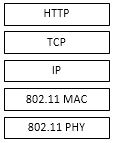
\includegraphics{intro/diagrams/tcpip.png}
	\caption{802.11 in the TCP/IP stack.}
\end{figure}

802.11 is split in to various task groups (TG) again which define extra amendments to the standard, the most prolific task groups are TGb, TGa, TGg and most recently TGn.

\begin{table}[htb!]
\begin{center}
	\begin{tabular}{| c | p{ 5cm } |}
		\hline
		\textbf{Task Group} & \textbf{Amendments} \\ \hline
		TGa & This amendment operates in the 5GHz band with a maximum data rate of 54Mbit/s, which allowed it to operate away from the noise of devices in the 2.4GHz band. This amendment is no longer valid. \\ \hline
		TGb & This brings throughput up to 11Mbit/s, and was implemented worldwide. Products that supported this amendment started to appear during 1999, starting with the Apple iBook \cite{intro:apple_ibook}. \\ \hline
		TGg & TGg allows for 54Mbit/s throughput in the 2.4GHz band, the same throughput as TGb. \\ \hline
		TGn & Allows for multiple antennas to increase the maximum data rate, getting up to 600Mbit/s when usng four spatial streams at a 40MHz channel width. \\ 
		\hline
	\end{tabular}
\end{center}
\end{table}

\subsubsection{802.11 Key Terms}

The 802.11 specification defines a number of components that make up various network architectures \cite{intro:80211_lecture}, which shall be referenced through the document.

\subsubsection*{Station}
A device that has the ability to connect to the wireless access point using the 802.11 protocol. For example, a desktop PC, laptop, smart phone, etc. The specification formally defines a station as:

\begin{center}
\quote Any device that contains an IEEE 802.11-conformant medium access control (MAC) and physical layer (PHY) interface to the wireless medium (WM).
\end{center}

Station is often interchangeably referred to as a node or client and can be either fixed, or mobile.

\subsubsection*{Access Point}
Access points are, more often than not, dedicated hardware devices that act as the central receiver and transmitter of a wireless network. Some wireless adapters have the ability to act as soft access points, which is how, for example, smartphones are able to become hotspots for devices without an internet connection.

\subsubsection*{Base Service Set(Base Service Set)}
A BSS is a group of stations that are connected to an access point which is connected to a wired network.

\begin{figure}[htb!]

\centering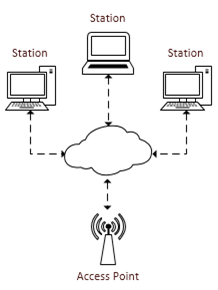
\includegraphics{intro/diagrams/bss.png}
\caption{An example BSS.}

\end{figure}
\newpage
\subsubsection*{Base Service Set Identification (BSSID)}
The unique identifier given to a BSS, in an infrastructure BSS this is the MAC address of the access point. In an ad hoc network (IBSS), with no governing access point, it is random and administered by the starting station \cite{intro:ieee_tutorial}.

\subsubsection*{Service Set Identification (SSID)}
The human readable  string given to a BSS, chosen by the access point, that is broadcasted in beacon and probe frames.
\newpage 
\begin{figure}[htb!]
\centering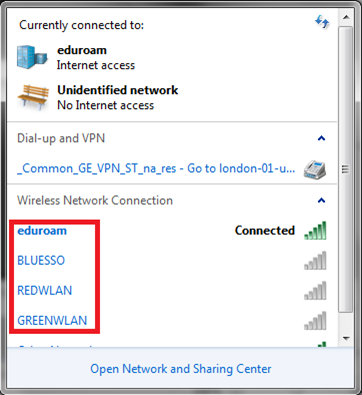
\includegraphics{intro/diagrams/ssid.png}
\caption{An SSID as displayed in Windows network manager.}
\end{figure}

\subsubsection*{Extended Service Set (ESS)}
An ESS is a group of two or more infrastructure BSS that share the same SSID and security credentials where the access points communicate to forward traffic and the movement of stations between the BSSs. This communication is performed by the distribution system (DS), which is out of the scope this report.

\begin{figure}[htb!]
\centering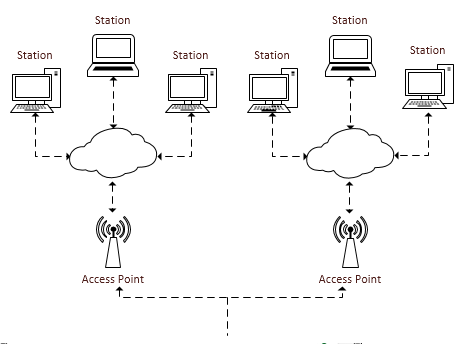
\includegraphics{intro/diagrams/ess.png}
\caption{Two BSS making an ESS.}
\end{figure}
\newpage

\subsubsection{802.11 Security}

The 802.11 is an inherently insecure \cite{intro:80211_lecture} base on which a large majority of enterprise applications are founded upon. Attempts have been made to secure networks by using various types of encryption, for example Wired Equivalent Policy (WEP) \cite{intro:netgear_wep} and WiFi Protected Access (WPA) \cite{intro:wiki_wpa}, however these standards only encrypt the data portion of the exchange. Management frames are left open and unencrypted which offers opportunity for exploitation in a number of ways- in which I go in to more detail in section \ref{sec:attacks}- from getting unsuspecting users to connect to a faked access point (page \pageref{sec:spoofap}) to collecting data based on access points a mobile device has connected to through the period beacon frames (page \pageref{sec:honeypot}).
 
\subsubsection{Leaky Applications}

There have been reports recently of applications written for Android that have been collecting and sending data to advertisers  \cite{intro:bbc_flashlight_app}, from what is perceived as innocuous information such as phone model and screen size, to personal data including, but not limited to, current location information, gender and date of birth, then at the extreme end entire contact lists. It has come to light, from the documents leaked by Edward Snowden, that GCHQ and the NSA have been targeting apps that send this type of data, unencrypted, back to advertisers as it allows them to build a profile of the user \cite{intro:angry_leak}. This profile can be built using similar methods to the Evercookie \cite{intro:evercookie}, that works on the premise of collecting as much information as it can about the user and hashing this so that it gives a unique identifier for the user. Methods such as this prove effective when attempting to circumvent UK cookie laws, by tracking users through fingerprinting methods.

\subsubsection{Profiling Users}

Fingerprinting is achieved by collecting as much information as you can about the user through commonly available methods, and then hashing the data and storing it either in a local database- or through a persistent cookie such as the Evercookie \cite{intro:evercookie}. It has been noted that if a user has Flash and Java enabled, the success rate of uniquely identifying is 94\% \cite{intro:unique_browser}. 

Interestingly, a paper \cite{intro:twitter_home_location} came out recently that documented the process they took in identifying the geo-location of Twitter users that did not include geotags by comparing the information in the content, hashtags, foursquare \cite{intro:foursquare_site} check-ins, locational references, etc. to those that had geotags \cite{intro:twitter_location_howto} in them. They found that, when omitting users identified as travelling, they could predict the home location from tweets to 68\% for cities, 70\% for states, 80\% for time-zones and 73\% for regions. This style of data mining highlights the effect that other users sharing personal location information can have on those that chose to omit the data \cite{intro:not_personal}. 

One of the golden nuggets, according to the NSA \cite{intro:angry_leak}, of unencrypted data is a photo upload, ideally to social media, but any endpoint will do. The reason for this is the Exif \cite{intro:exif_wiki} tag data that accompanies the photograph. This can detail various pieces of information on modern smartphones with a GPS chip, but most importantly it contains the make and model, datetime stamp and GPS location \cite{intro:wiki_geotag}. These fields are often added by default. 
\begin{center}
[Picture from Exif app of extracted data]
\end{center}
Social media websites, such as Facebook and Twitter, strip any Exif data \cite{intro:twitter_exif} from uploaded photos in an attempt to preserve the privacy of their users. This can be effective at stopping their users from taking data from photos; however, depending on when during the upload process this takes place it is still susceptible to wiretapping (referring here to both a MITM attack and by public entities at locations they would have access to \cite{intro:room_641a}) if the user is not transmitting over HTTPS. 

Wiretapping in this instance can refer to either a higher body monitoring traffic, or a malicious user performing a man in the middle attack on the wireless network. If, for example, the photo is sanitized on the client side, this means that Exif data is not transmitted and is not susceptible to wiretapping; however, if this action is performed server side, for example by using PHP to create a new image from the old one, then the Exif data is transmitted and is open to monitoring. There is an argument brewing in creative industries that stripping the Exif data destroys any copyright information the picture may be able to carry as they often manage this data to allow them to detect when their image is being used without their permission.

There has been a recent shift to move to forcing HTTPS by default on websites as a way of deterring Joe Bloggs from attempting attacks on open encrypted networks. It encrypts any traffic to and from the client using SSL, and prevents MITM attacks, although if HTTPS is only used during the login stage of a website to gain access, and then reverts back to HTTP and sends session data, the session can still be hijacked.

Angry Birds hit the headlines when it was named in one of the NSA/GCHQ releases as an application they can exploit to gain user data. Being an incredibly popular game, it demonstrates the ease in which users can be coerced into allowing applications access to their data.

\subsubsection{Culmination}

This project takes inspiration from the information detailed above. It sets out to develop an application that analyses probe request frames and sends spoofed probe response frames in order to establish itself as an access point for any devices that have previously connected to unencrypted networks. Alongside this an Android game will be developed that intentionally leaks personal and location data unencrypted across the network. This will then be combined with the first application to demonstrate how apps can broadcast your personal data, unknowing to you, to an attacker as you pass by.

\subsection{Objectives}
This aim of this project to expose the inherent security vulnerability that unencrypted networks leave behind on a mobile wireless device's preferred network list whilst they pass by in the pocket of the owner. This will be achieved by developing software capable of responding to 802.11 probe request frames emitted by roaming smartphones in an attempt to masquerade as the requested access point. To solidify the point, a leaky Android application will send personal data and location data to a server unencrypted, which can then be monitored by the application or wireshark.

Once a connection with a device has been established the laptop running the software will create a bridge between the soft access point and the hardware to allow for traffic to pass normally, and HTTP traffic to be analysed. The security vulnerabilities will be demonstrated by an Android game, similar to one in the top charts currently, that has been written with the sole intention of leaking data. 

Finally, I want to look into what steps can be taken to prevent this attack happening at root level, and the possible ways of adding security at application level to notify users of hijacking attempts.

\subsection{Content}
<some>
\clearpage